% !TEX program = xelatex
\documentclass[11pt,a4paper]{article}
\usepackage{fontspec}
\setmainfont{Calibri}
\setmonofont[Scale=0.88]{Consolas}
\usepackage{polyglossia}\setdefaultlanguage{polish}
\usepackage[table]{xcolor}
\usepackage{booktabs,tabularx,longtable,array,geometry,enumitem,graphicx,fancyhdr,caption}
\usepackage[most]{tcolorbox}
\usepackage{listings}
\PassOptionsToPackage{hyphens}{url}
\usepackage[hidelinks,unicode]{hyperref}
\emergencystretch=2.5em
\geometry{a4paper,margin=2.1cm,top=2.3cm,bottom=2.3cm}
\setlength{\parindent}{0pt}\setlength{\parskip}{5pt}
\definecolor{apteal}{HTML}{0E7C86}
\definecolor{apteallight}{HTML}{E6F4F5}
\definecolor{apgrey}{HTML}{F3F4F6}
\definecolor{apamber}{HTML}{B45309}
\definecolor{apamberlight}{HTML}{FEF3C7}
\definecolor{apred}{HTML}{B91C1C}
\definecolor{apredlight}{HTML}{FEE2E2}
\definecolor{apgreen}{HTML}{15803D}
\definecolor{apgreenlight}{HTML}{DCFCE7}
\renewcommand{\arraystretch}{1.22}
\captionsetup{font=small,labelfont=bf}
\pagestyle{fancy}\fancyhf{}
\fancyfoot[L]{\small AMPERE POINT — TopAC EVE01-11R: specyfikacja i obsługa przez Wi-Fi · v1 · 2026-09-23}
\fancyfoot[R]{\small\thepage}
\renewcommand{\headrulewidth}{0pt}
\lstset{basicstyle=\ttfamily\small,breaklines=true,columns=fullflexible,keepspaces=true,frame=single,rulecolor=\color{apteal!40},backgroundcolor=\color{apgrey},xleftmargin=4pt,framexleftmargin=4pt}
\newtcolorbox{uwaga}[1][Uwaga]{enhanced,colback=apamberlight,colframe=apamber,title={#1},fonttitle=\bfseries,boxrule=0.6pt,arc=2pt,left=6pt,right=6pt,top=4pt,bottom=4pt}
\newtcolorbox{info}[1][Jak to działa]{enhanced,colback=apteallight,colframe=apteal,title={#1},fonttitle=\bfseries,boxrule=0.6pt,arc=2pt,left=6pt,right=6pt,top=4pt,bottom=4pt}
\newtcolorbox{wazne}[1][Ważne dla bezpieczeństwa]{enhanced,colback=apredlight,colframe=apred,title={#1},fonttitle=\bfseries,boxrule=0.6pt,arc=2pt,left=6pt,right=6pt,top=4pt,bottom=4pt}
\newtcolorbox{przyklad}[1][Przykład liczbowy]{enhanced,colback=apgreenlight,colframe=apgreen,title={#1},fonttitle=\bfseries,boxrule=0.6pt,arc=2pt,left=6pt,right=6pt,top=4pt,bottom=4pt}
\newcommand{\tagP}{\textcolor{apgreen}{\textbf{[P]}}}
\newcommand{\tagW}{\textcolor{apamber}{\textbf{[W]}}}
\newcommand{\code}[1]{\texttt{#1}}
\setlist{nosep,leftmargin=*}

\begin{document}

{\LARGE\bfseries TopAC Portable EV Charger 11 kW (EVE01-11R)\par}
{\Large Specyfikacja i instrukcja obsługi przez Wi-Fi\par}
\vspace{2pt}
{\small AMPERE POINT · dokument roboczy v1 · 23 września 2026 · oprac. Dawid Cękała\par}
\vspace{4pt}\textcolor{apteal}{\rule{\textwidth}{1.2pt}}

\section*{Jak czytać ten dokument}

Dokument opisuje ładowarkę TopAC EVE01-11R z linii „Powered by Shelly” tak, jak ją widzi użytkownik i integrator: co to jest, co potrafi, jak ją sparować, jak nią sterować z aplikacji, z przeglądarki i z własnego oprogramowania. Fakty pochodzą z pięciu źródeł: instrukcji producenta (wersja 251023, listopad 2025), karty katalogowej Shelly, dokumentacji API Shelly dla tego urządzenia, bazy wiedzy Shelly oraz z egzemplarza leżącego na biurku (zdjęcia w folderze \code{zdjecia}). Każde stwierdzenie, którego nie da się potwierdzić w dokumentacji, jest oznaczone:

\begin{itemize}
\item \tagP{} — potwierdzone w dokumentacji producenta albo Shelly,
\item \tagW{} — wniosek z analogii lub z obserwacji; do sprawdzenia na urządzeniu (lista testów jest w rozdziale~\ref{sec:testy}).
\end{itemize}

Przy każdej funkcji podaję mechanizm i, gdzie to ma sens, przykład liczbowy. Nazwy pól i poleceń programowych podaję dokładnie tak, jak występują w oprogramowaniu, bo są potrzebne do pracy; w opisach słownych używam zwykłych nazw.

\tableofcontents

\section{Czym jest to urządzenie}

TopAC EVE01-11R to przenośna ładowarka prądu przemiennego do samochodów elektrycznych: wtyk przemysłowy CEE 16~A trójfazowy po jednej stronie, złącze Typu~2 po drugiej, między nimi skrzynka sterująca z wyświetlaczem i jednym przyciskiem dotykowym. Fizycznie produkuje ją chińska firma Zhejiang Guangwei Electric \& Tools (marka handlowa TopAC, strona acdctop.com), a do Europy wprowadza Shelly Europe Ltd. jako importer \tagP.

To, co odróżnia ją od zwykłej chińskiej ładowarki, to moduł łączności: zamiast modułu Tuya siedzi w niej moduł platformy Shelly~X pracujący w trybie „XT1” (tryb, w którym producent dokłada do standardowego oprogramowania Shelly własną usługę napisaną w JavaScripcie) \tagP. Skutek jest taki, że ładowarka zachowuje się jak każde inne urządzenie Shelly: ma własny serwer WWW, lokalne API, Bluetooth, MQTT, skrypty i harmonogramy zapisane w samym urządzeniu, a chmura jest dodatkiem, nie warunkiem działania.

\begin{info}[Podział ról w środku]
W skrzynce są dwa „mózgi”. Mikrokontroler producenta pilnuje bezpieczeństwa i rozmawia z samochodem (sygnał Control Pilot, przekaźniki, pomiary, kody błędów). Moduł Shelly rozmawia ze światem (Wi-Fi, Bluetooth, aplikacja, chmura, API) i wymienia z mikrokontrolerem krótkie komunikaty po łączu szeregowym. Dlatego w API ładowarki widać z jednej strony standardowe usługi Shelly (Wi-Fi, MQTT, harmonogramy), a z drugiej sześć „wirtualnych komponentów”, które są w istocie odbiciem danych mikrokontrolera: stan, prąd, energia, czas, telemetria faz i polecenie start/stop.
\end{info}

\section{Specyfikacja techniczna}

\subsection{Parametry elektryczne i mechaniczne \tagP}

\begin{tabularx}{\textwidth}{>{\bfseries}p{4.6cm}X}
\toprule
Model & EVE01-11R (EAN 3800238071448) \\
Zasilanie & 3-fazowe 400~V AC (dopuszczalnie 220/380–240/415~V), 50/60~Hz, sieci TN-C i TN-S \\
Wtyk sieciowy & CEE 16~A, 5-stykowy, trójfazowy (czerwony) \\
Prąd ładowania & 6–16~A, nastawialny (przyciskiem lub z aplikacji) \\
Moc maksymalna & 11~kW (3 × 16~A × 230~V) \\
Złącze pojazdu & Typ~2 wg EN~62196 \\
Długość całkowita & 5,6~m wg instrukcji (karta katalogowa Shelly podaje 5~m) \\
Przewód wejściowy & 5 × 2,5~mm² + 2 × 0,5~mm² \\
Przewód wyjściowy & 5 × 2,5~mm² + 1 × 0,5~mm² \\
Rezystancja izolacji przewodu & > 1000~MΩ przy 500~V DC \\
Ochrona różnicowoprądowa & RCD typu A 30~mA + wykrywanie składowej stałej 6~mA DC \\
Zabezpieczenia & przepięciowe, podnapięciowe, nadprądowe, termiczne (skrzynka i wtyk), upływowe, zwarciowe, zwarcie diody CP, sklejenie przekaźnika, brak uziemienia, ochrona przed przepięciami atmosferycznymi \\
Stopień ochrony & IP65 (skrzynka sterująca) \\
Temperatura pracy & −25~°C do +45~°C \\
Temperatura składowania & −40~°C do +70~°C, wilgotność ≤ 95~\% \\
Wysokość n.p.m. & do 2000~m \\
Zalecane zabezpieczenie obwodu & wyłącznik 3-fazowy 20~A charakterystyki B lub C, alternatywnie 3 × 20~A gG; przewód zasilający 4~mm² przy długości do 50~m \\
Łączność & Wi-Fi 802.11 b/g/n 2,4~GHz, Bluetooth 5 \\
Normy badań & EN IEC 62752, EN IEC 62196, EN 50620 / IEC 62893 \\
Deklaracja zgodności & RED 2014/53/UE, RoHS 2011/65/UE; pełny tekst: \url{https://shelly.link/greatway-evc11-doc} \\
\bottomrule
\end{tabularx}

\begin{uwaga}[Dwie wartości długości przewodu]
Instrukcja producenta mówi o 5,6~m, karta katalogowa Shelly o 5~m, a jeden ze sklepów o 4,7~m przewodu do samochodu. Najprawdopodobniej to trzy sposoby mierzenia tej samej rzeczy (z wtykami lub bez, sam odcinek do auta lub całość). Do porównań z Q11 przyjmuję 5,6~m całkowitej długości i warto to zmierzyć taśmą \tagW.
\end{uwaga}

\subsection{Co siedzi w oprogramowaniu \tagP}

Dokumentacja API Shelly wymienia dla tego urządzenia następujące standardowe usługi: System, XMOD service, Wi-Fi, Bluetooth Low Energy, Schedule (harmonogramy), Cloud, MQTT, Outbound Websocket, Webhook, KVS (mała pamięć klucz-wartość), HTTP. Do tego obsługę czujników Bluetooth w standardzie BTHome (ładowarka może być bramką dla czujników Shelly BLU) oraz sześć wirtualnych komponentów, które są sednem tego urządzenia:

\begin{tabularx}{\textwidth}{>{\ttfamily}p{3.1cm}p{2.1cm}p{1.9cm}X}
\toprule
\textrm{\textbf{Komponent}} & \textbf{Typ} & \textbf{Dostęp} & \textbf{Znaczenie} \\
\midrule
work\_state & enum & odczyt & stan ładowarki (wolna, czeka, ładuje, pauza, …) \\
current\_limit & number & odczyt/zapis & nastawa prądu ładowania w amperach \\
phase\_info & object & odczyt & napięcie, prąd i moc każdej fazy, sumy oraz energia całkowita (kWh) \\
start\_charging & boolean & odczyt/zapis & start (true) lub stop (false) sesji \\
energy\_charge & number & odczyt & energia bieżącej sesji (kWh) \\
time\_charge & number & odczyt & czas trwania sesji (w przykładzie z dokumentacji wartość 128; jednostka minuty \tagW) \\
\bottomrule
\end{tabularx}

Oraz konfigurację usługi (\code{Service.GetConfig}, id 0), czyli ustawienia, które w aplikacji widać jako przełączniki:

\begin{tabularx}{\textwidth}{>{\ttfamily}p{5.5cm}p{1.5cm}X}
\toprule
\textrm{\textbf{Pole}} & \textbf{Typ} & \textbf{Znaczenie} \\
\midrule
auto\_balance.enable & boolean & włącza dynamiczne równoważenie obciążenia (Auto Balance) \\
auto\_balance.em\_ip & string & adres IP licznika Shelly EM w sieci lokalnej (wymagany, gdy enable = true) \\
auto\_balance.max\_current & number & dopuszczalny prąd całkowity domu razem z ładowarką, w amperach (fabrycznie 24) \\
auto\_balance.exclude\_self\_current & boolean & czy odjąć prąd ładowarki od odczytu licznika (gdy licznik „widzi” też ładowarkę); fabrycznie true \\
auto\_charge & boolean & start automatyczny po wpięciu wtyczki (fabrycznie true) \\
global\_charge\_limit & number & limit energii sesji, 0–1000~kWh (null = brak) \\
global\_time\_limit & number & limit czasu sesji, 0–1440~min (null = brak) \\
\bottomrule
\end{tabularx}

\subsection{Zestawienie możliwości w jednym miejscu}

\begin{tabularx}{\textwidth}{p{5.2cm}Xc}
\toprule
\textbf{Funkcja} & \textbf{Zakres / uwagi} & \textbf{Źródło} \\
\midrule
Nastawa prądu & 6–16~A; z przycisku tylko w pierwszych 3 minutach po włączeniu, z aplikacji i API zawsze & \tagP \\
Start/stop zdalny & tak, z aplikacji i API; przy wyłączonym auto-starcie ładowanie rusza dopiero po autoryzacji z aplikacji & \tagP \\
Limit energii na sesję & 0–1000~kWh; po osiągnięciu sesja się kończy, wznowienie wymaga przepięcia wtyczki & \tagP \\
Limit czasu na sesję & 0–1440~min; jak wyżej, oba limity mogą działać naraz & \tagP \\
Harmonogramy & w urządzeniu, do 20 zadań po 5 poleceń, składnia cron z sekundami, wschód/zachód słońca & \tagP \\
Auto Balance & wymaga licznika Shelly EM Gen2/Pro lub nowszego w tej samej sieci Wi-Fi; rezerwa 2~A; dwa tryby & \tagP \\
Skrypty JavaScript & w urządzeniu (rodzina XMOD: do 10 instancji) & \tagP \\
API lokalne & HTTP GET/POST JSON-RPC, MQTT, WebSocket wychodzący, webhooki & \tagP \\
Bluetooth & parowanie, bramka BTHome dla czujników BLU & \tagP \\
Chmura & Shelly Cloud (Europa), aplikacja Shelly Smart Control, opcjonalna & \tagP \\
Home Assistant & natywna integracja Shelly; wirtualne komponenty number/enum/boolean są obsługiwane & \tagP \tagW \\
Wyświetlacz & segmentowy: ikony, prąd/energia, pasek stanu, kod błędu & \tagP \\
\bottomrule
\end{tabularx}

\section{Panel, wyświetlacz i przycisk}

\subsection{Elementy wyświetlacza \tagP}

\begin{figure}[h]
\centering
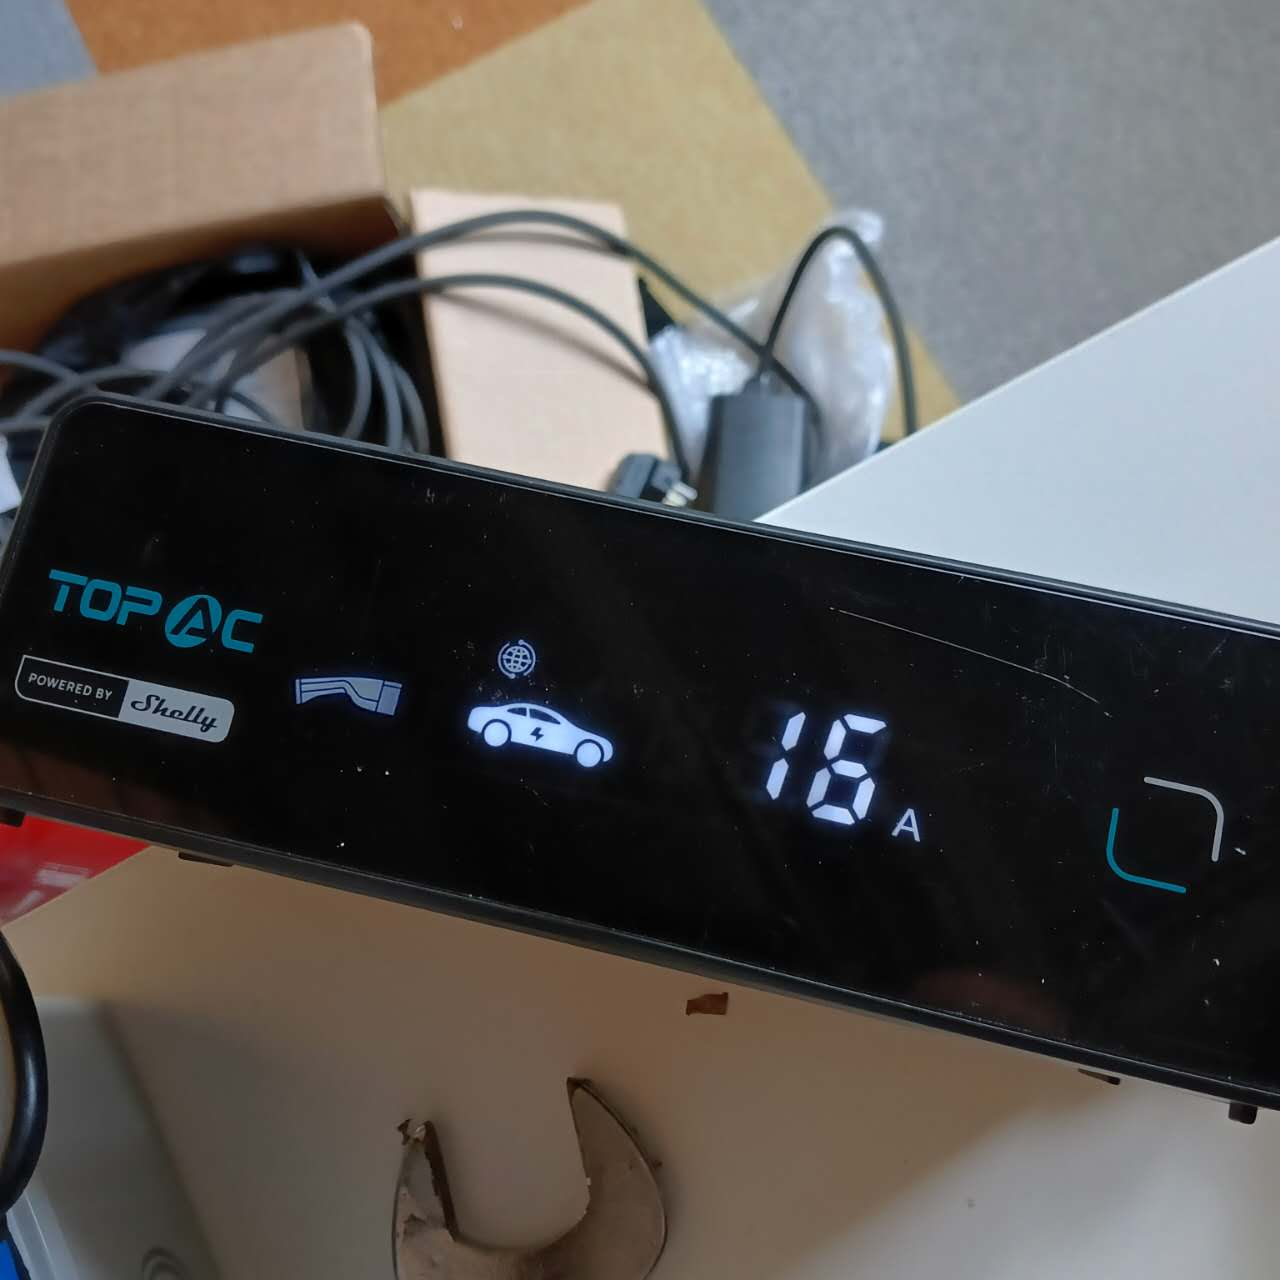
\includegraphics[width=0.32\textwidth]{zdjecia/stany_ladowania/A.jpg}\hfill
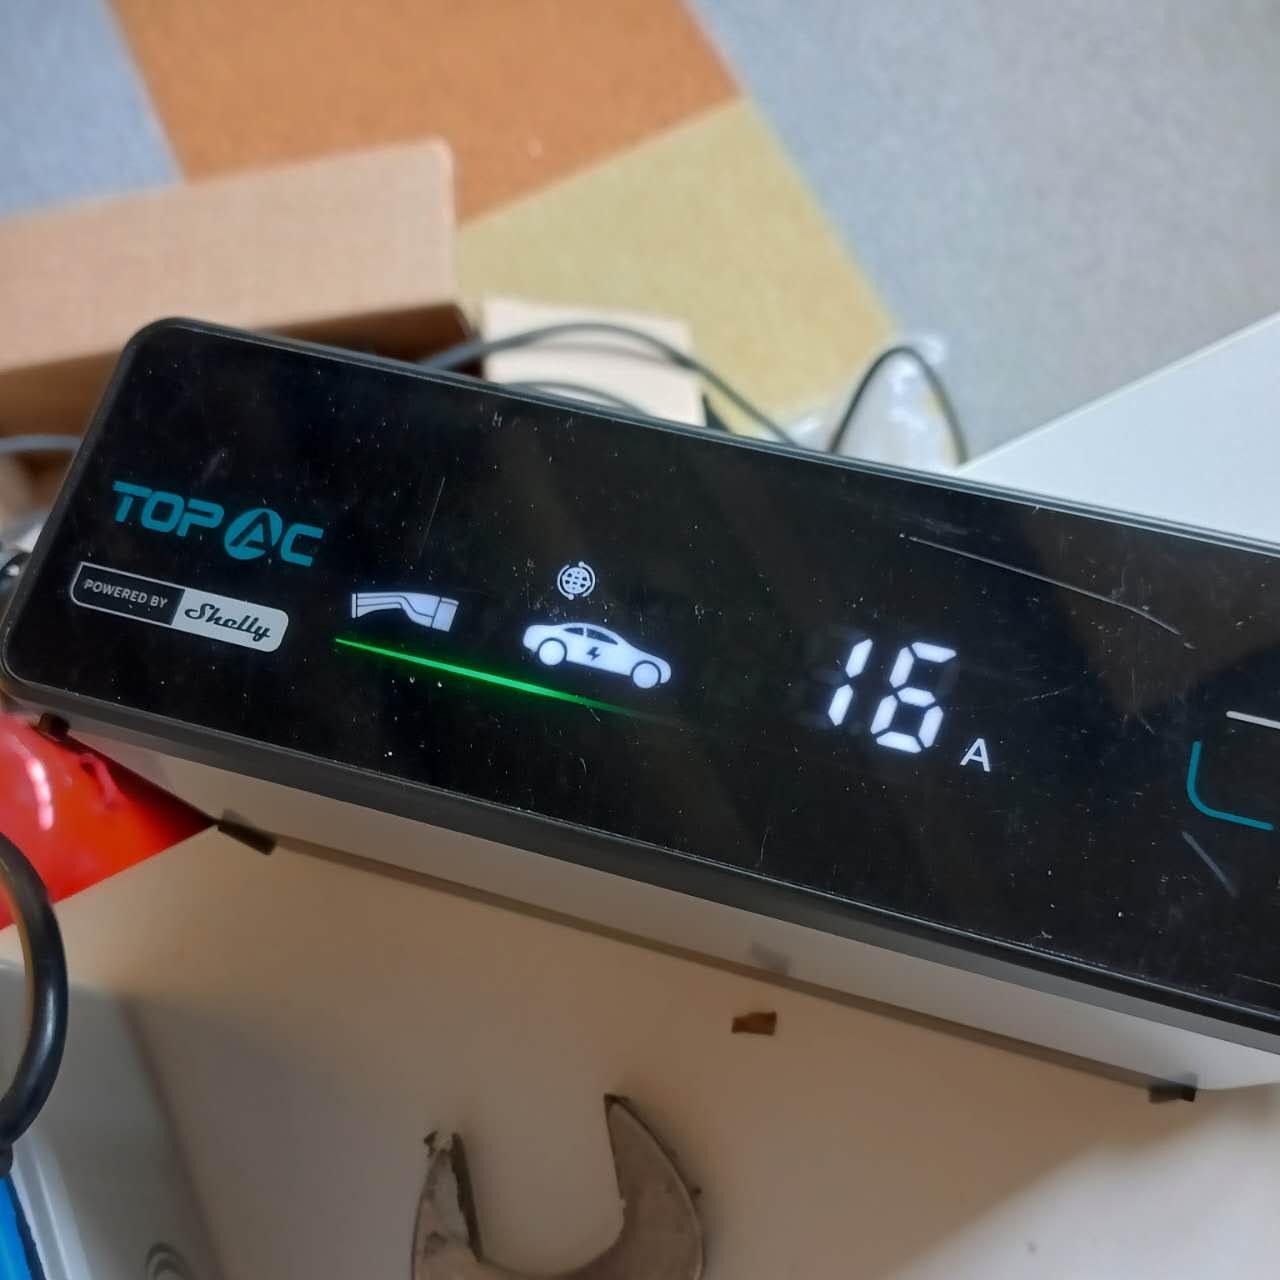
\includegraphics[width=0.32\textwidth]{zdjecia/stany_ladowania/B.jpg}\hfill
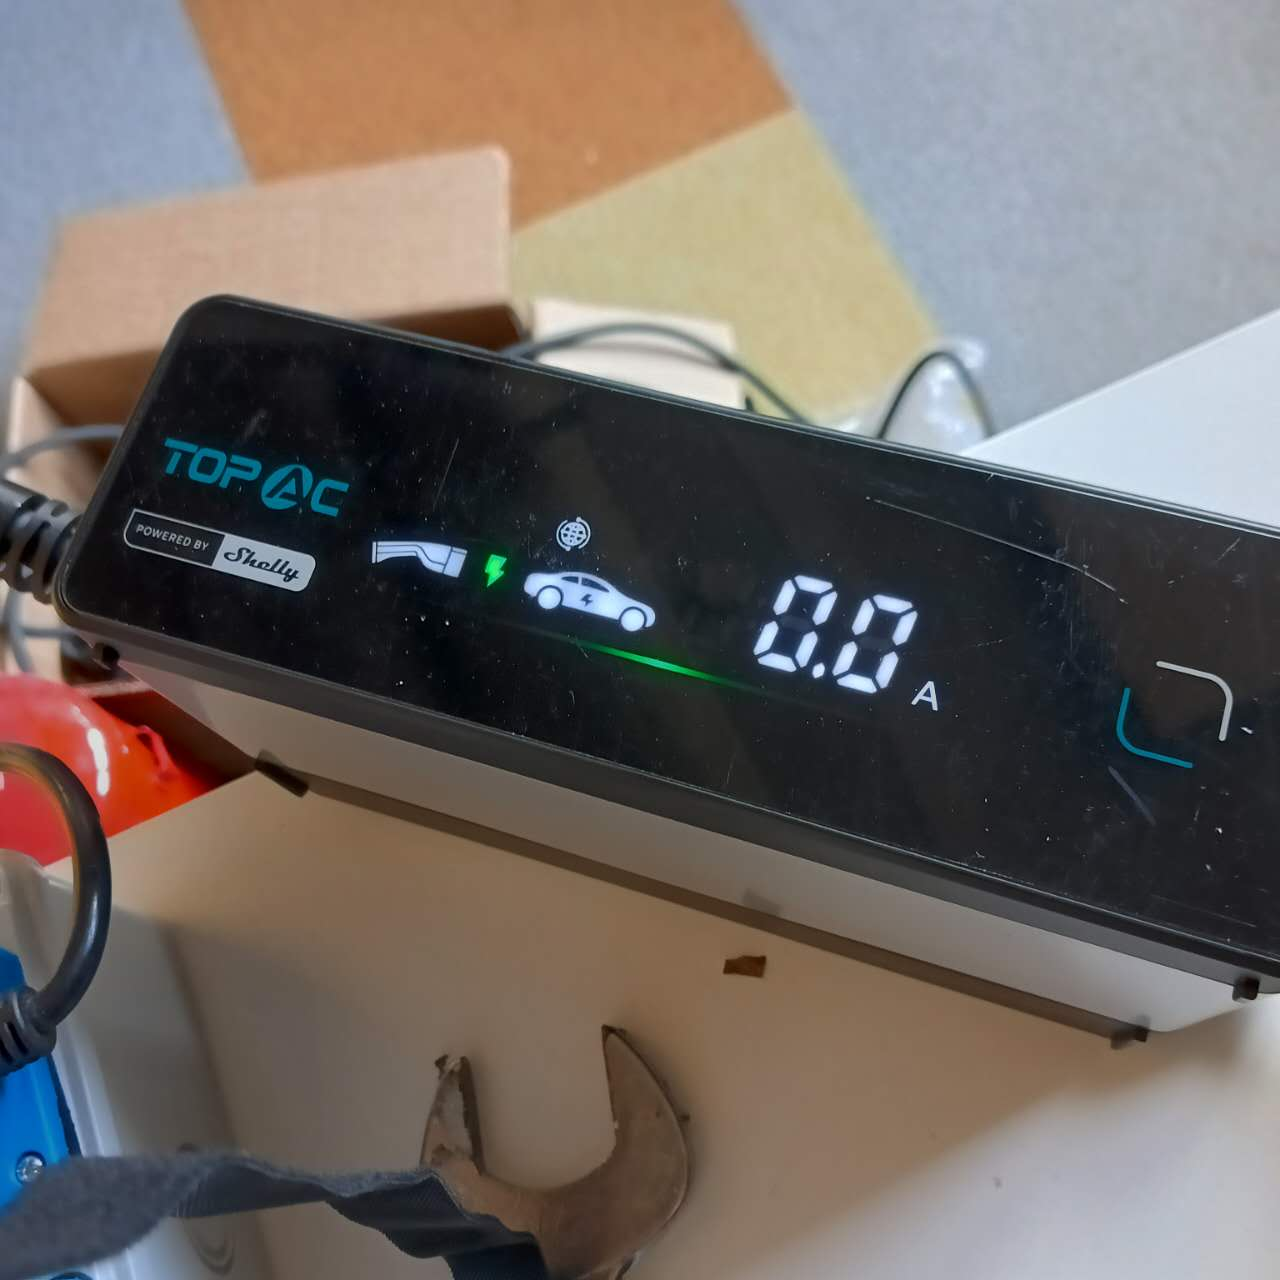
\includegraphics[width=0.32\textwidth]{zdjecia/stany_ladowania/C.jpg}
\caption{Egzemplarz na biurku w trzech stanach sygnału Control Pilot: A (brak pojazdu), B (pojazd podłączony), C (pojazd gotowy, ładowanie). Zdjęcia własne z symulatorem pojazdu.}
\end{figure}

\begin{tabularx}{\textwidth}{p{4.2cm}X}
\toprule
\textbf{Element} & \textbf{Znaczenie} \\
\midrule
Przycisk dotykowy (prawy skraj) & jedyny element obsługi na urządzeniu: wybór prądu, reset sieci \\
Cyfry z jednostką A / kWh & podczas ładowania: bieżący prąd; po zakończeniu: energia ostatniej sesji w kWh; w spoczynku: nastawiony prąd (obserwacja: „16~A” w stanie A i B) \tagW \\
Ikona złącza (wtyczka) & miga: można wpiąć wtyczkę do auta; świeci stale: wtyczka jest w gnieździe pojazdu \\
Zielona błyskawica przy ikonie złącza & pojazd gotowy do ładowania (po uzgodnieniu sygnału Control Pilot) \\
Ikona samochodu z błyskawicą & symbol pojazdu; na naszym egzemplarzu nad nią widać ikonę kuli ziemskiej, której instrukcja nie opisuje; najpewniej sygnalizuje łączność z siecią lub chmurą \tagW \\
Pasek stanu pod ikonami & zielony stały: czuwanie lub ładowanie zakończone; zielony „wydłużający się”: ładowanie trwa; czerwony stały: błąd (razem z migającym trójkątem i kodem E\ldots) \\
Trójkąt ostrzegawczy & miga przy błędzie; kod błędu pojawia się w polu cyfr (tabela w rozdziale~\ref{sec:bledy}) \\
\bottomrule
\end{tabularx}

Zdjęcia potwierdzają ten opis: w stanie B pojawia się stały zielony pasek (czuwanie z podłączonym autem), w stanie C dochodzi zielona błyskawica, a pole cyfr przełącza się z nastawy „16~A” na bieżący prąd „0,0~A” (symulator nie pobiera prądu, więc zero jest poprawne).

\subsection{Przycisk \tagP}

\begin{tabularx}{\textwidth}{p{4.2cm}X}
\toprule
\textbf{Gest} & \textbf{Skutek} \\
\midrule
Krótkie naciśnięcie & zmiana nastawy prądu ładowania (kolejne wartości z zakresu 6–16~A; krok 1~A \tagW) \\
Przytrzymanie 6~s & „reset sieci”: włącza punkt dostępowy Wi-Fi i Bluetooth urządzenia; pasek stanu miga na zielono, urządzenie jest gotowe do parowania \\
\bottomrule
\end{tabularx}

\begin{uwaga}[Okno trzech minut]
Ze względów bezpieczeństwa \emph{wszystkie} operacje ręczne na urządzeniu, łącznie ze zmianą prądu przyciskiem, są możliwe tylko przez pierwsze 3 minuty po włączeniu zasilania. Po tym czasie przycisk nie reaguje; zmiany robi się z aplikacji lub z przeglądarki, albo przepina się wtyk sieciowy, żeby otworzyć okno na nowo. To decyzja produktowa, nie ograniczenie techniczne: chroni przed manipulacją prądem przez osoby postronne przy ładowarce zostawionej na parkingu. Ładowarka pamięta ostatnią nastawę prądu i używa jej w następnej sesji.
\end{uwaga}

\section{Pierwsze uruchomienie i parowanie}

\subsection{Zanim zaczniesz}

\begin{itemize}
\item Sieć Wi-Fi 2,4~GHz w zasięgu miejsca, gdzie ładowarka będzie pracować (pasmo 5~GHz nie jest obsługiwane) \tagP.
\item Telefon z włączonym Bluetooth i zainstalowaną aplikacją \textbf{Shelly Smart Control} (App Store, Google Play, AppGallery); aplikacja jest bezpłatna, wymaga założenia konta \tagP.
\item Gniazdo CEE 16~A z poprawnym uziemieniem; bez uziemienia ładowarka zgłosi błąd E13 i nie ruszy \tagP.
\end{itemize}

\subsection{Sposób 1: przez Bluetooth (zalecany przez producenta) \tagP}

\begin{enumerate}
\item Wepnij ładowarkę do gniazda CEE i poczekaj na uruchomienie wyświetlacza.
\item Przytrzymaj przycisk 6~s. Pasek stanu zacznie migać na zielono: punkt dostępowy i Bluetooth są aktywne. (W urządzeniach Shelly punkt dostępowy i Bluetooth są też aktywne automatycznie przez 15 minut od włączenia zasilania; przytrzymanie przycisku otwiera to okno ponownie.)
\item W aplikacji dotknij „+” w prawym dolnym rogu ekranu.
\item Wybierz „Add via Bluetooth” (dodaj przez Bluetooth) i „Next”; pojawi się lista wykrytych urządzeń.
\item Wybierz ładowarkę i „Next”.
\item Wpisz nazwę i hasło swojej sieci Wi-Fi i dotknij „Add device”.
\item Poczekaj, aż aplikacja skończy (może to potrwać kilka minut). Pojawi się komunikat o powodzeniu.
\item Nadaj urządzeniu nazwę i wybierz obrazek, „Next”.
\item Wybierz pomieszczenie albo utwórz nowe („Add room”).
\item „Save”. Ładowarka jest na koncie.
\end{enumerate}

\subsection{Sposób 2: przez punkt dostępowy Wi-Fi ładowarki \tagP}

Każde urządzenie Shelly po włączeniu (i po przytrzymaniu przycisku) rozgłasza własną sieć Wi-Fi o nazwie w schemacie \code{NazwaUrządzenia-XXXXXXXXXX}, gdzie XXXXXXXXXX to unikalny identyfikator. W dokumentacji API tej ładowarki identyfikator ma postać \code{evcharger-543204516524}, więc sieci należy szukać pod nazwą zaczynającą się od \code{EVCharger-} lub \code{evcharger-} \tagW.

\begin{enumerate}
\item Na telefonie lub laptopie połącz się z tą siecią.
\item W przeglądarce wpisz \code{http://192.168.33.1}. Otworzy się lokalny interfejs ładowarki.
\item W sekcji sieci (Networks → Wi-Fi) wpisz nazwę i hasło domowej sieci i zapisz. Ładowarka przełączy się do domowej sieci i dostanie adres z routera.
\item Jeśli chcesz mieć ją także w aplikacji: „+” → „Add via Wi-Fi (AP scan)” albo „Scan network” (skanowanie sieci lokalnej), dalej jak wyżej.
\end{enumerate}

Po dodaniu do aplikacji punkt dostępowy ładowarki jest wyłączany, żeby nikt postronny nie mógł się do niej dostać. Można go włączyć ponownie w ustawieniach sieci (zakładka Networks → Access Point), najlepiej z hasłem \tagP.

\begin{uwaga}[Adres w sieci domowej]
Do sterowania z własnego oprogramowania (rozdział~\ref{sec:api}) ładowarka musi mieć stały adres IP. Najprościej zarezerwować go w routerze (rezerwacja DHCP po adresie MAC), zamiast wpisywać adres statyczny w ładowarce. Adres i wersję oprogramowania odczytasz w aplikacji w ustawieniach urządzenia albo w stopce lokalnego interfejsu.
\end{uwaga}

\subsection{Aktualizacja oprogramowania \tagP}

Ładowarka przyjeżdża z oprogramowaniem fabrycznym; Shelly udostępnia aktualizacje bezpłatnie, przez aplikację albo lokalny interfejs (Settings → Firmware). Instrukcja producenta przerzuca odpowiedzialność za instalowanie aktualizacji na użytkownika. Praktyczna rada: przed testami API zaktualizować, bo funkcje sterowania prądem z zewnątrz pojawiały się w kolejnych wersjach (rozdział~\ref{sec:api}, ostrzeżenie o forum).

\section{Obsługa z aplikacji Shelly Smart Control}

\subsection{Ładowanie krok po kroku \tagP}

\begin{enumerate}
\item Wepnij wtyk CEE do gniazda.
\item Ustaw prąd: przyciskiem (w oknie 3 minut) albo w aplikacji.
\item Wepnij złącze Typu~2 do auta. Ikona złącza przestaje migać.
\item Gdy auto zgłosi gotowość, przy ikonie złącza pojawia się zielona błyskawica.
\item Ładowanie rusza samo po uzgodnieniu z autem (jeśli auto-start jest włączony).
\item Zakończenie: zatrzymaj sesję z auta albo z aplikacji, zwolnij blokadę wtyczki w aucie, wyjmij złącze, dopiero potem wtyk CEE.
\end{enumerate}

\begin{wazne}
Nie wyjmuj wtyku CEE z gniazda podczas ładowania. Pod obciążeniem 16~A na fazę styki wtyku łukują; instrukcja producenta zakazuje tego wprost.
\end{wazne}

\subsection{Auto charge: start automatyczny albo po autoryzacji \tagP}

Fabrycznie włączony. Gdy jest włączony, sesja rusza sama po wpięciu i zgłoszeniu gotowości przez auto. Gdy go wyłączysz w aplikacji, ładowarka \emph{nie} zacznie ładować, dopóki nie zatwierdzisz sesji w aplikacji. To najprostsza forma autoryzacji: ładowarka na wspólnym parkingu ładuje tylko wtedy, gdy właściciel kliknie „start”.

\begin{info}[Dlaczego ładowarka „mrugnie” dwiema sekundami ładowania]
Przy wyłączonym auto-starcie ładowarka po wpięciu auta i tak uruchamia krótką, dwusekundową sesję. Producent tłumaczy to dwiema rzeczami: niektóre samochody zgłaszają błąd, jeśli po podłączeniu nie zobaczą żadnego ładowania, a poza tym dopiero po tym „uścisku dłoni” harmonogramy i Auto Balance mają z czym pracować. Dla użytkownika to nieistotne; dla integratora ważne, bo w logu pojawi się krótka sesja z energią bliską zera.
\end{info}

\subsection{Limity sesji \tagP}

\begin{itemize}
\item \textbf{Global charge limit} — maksymalna energia jednej sesji w kWh (0–1000).
\item \textbf{Global time limit} — maksymalny czas jednej sesji w minutach (0–1440).
\end{itemize}

Oba mogą być aktywne naraz; sesja kończy się, gdy pierwszy z nich zostanie osiągnięty, a w stanie ładowarki pojawia się flaga. Żeby ładować dalej, trzeba wypiąć i wpiąć złącze Typu~2: limit dotyczy sesji, a sesję zamyka fizyczne rozłączenie.

\begin{przyklad}[Limit energii jako „doładuj 100 km”]
Auto zużywa 18~kWh na 100~km. Ustawiasz limit energii 18~kWh i prąd 16~A: ładowarka odda 18~kWh w około 1~h 40~min (11~kW × 1,64~h = 18~kWh) i sama przestanie. Ten sam efekt bez limitu wymagałby pilnowania aplikacji.
\end{przyklad}

\subsection{Harmonogramy \tagP}

W aplikacji (i w lokalnym interfejsie) tworzy się harmonogramy start/stop ładowania o zadanej godzinie w wybrane dni. Harmonogramy są zapisane w ładowarce i działają bez internetu. Obsługują też pory względem wschodu i zachodu słońca (wymaga ustawienia lokalizacji urządzenia). Techniczny opis i przykład tworzenia harmonogramu z API jest w rozdziale~\ref{sec:api}.

\subsection{Auto Balance: dynamiczne równoważenie obciążenia \tagP}

\textbf{Co robi.} Ładowarka co chwilę pyta licznik energii Shelly (przez sieć Wi-Fi) o prąd pobierany przez cały dom i tak dobiera własny prąd, żeby suma nie przekroczyła nastawionego limitu całkowitego (Total current limit). W obliczeniu jest zawsze rezerwa 2~A.

\textbf{Czego wymaga.} Licznika Shelly EM generacji 2 lub Pro albo nowszego (Shelly Pro 3EM, 3EM-63T, 3EM-63W) zainstalowanego w rozdzielnicy, w tej samej sieci Wi-Fi co ładowarka, z aktualnym oprogramowaniem. W dostawie od Shelly licznika nie ma (jest zapowiedziany przekładnik 120~A, który bez licznika nic nie zmierzy), więc do testu Auto Balance trzeba dokupić licznik lub poprosić Shelly.

\textbf{Dwa tryby.} Zależą od tego, czy licznik „widzi” prąd ładowarki:
\begin{itemize}
\item tryb domyślny: ładowarka jest podłączona za licznikiem, więc licznik mierzy dom razem z ładowarką; ładowarka odejmuje własny prąd od odczytu, żeby nie liczyć go dwa razy (pole \code{exclude\_self\_current} = true);
\item tryb drugi: ładowarka jest podłączona przed licznikiem (licznik jej nie widzi); w aplikacji odznacza się pole „The consumption of the EV charger is included in the measured current reported from the EM”.
\end{itemize}

\textbf{Zachowanie przy awarii.} Jeśli ładowarka trzy razy z rzędu nie dostanie odpowiedzi od licznika, przerywa ładowanie i wyłącza Auto Balance. To bezpieczne zachowanie (lepiej nie ładować niż przeciążyć przyłącze), ale trzeba o nim wiedzieć: słabe Wi-Fi w garażu skończy się przerwanymi sesjami.

\begin{przyklad}[{Przyłącze 3 × 25 A, limit 25 A}]
Dostępny prąd dla ładowarki = limit − rezerwa − pobór domu = 25 − 2 − pobór domu.
\begin{itemize}
\item Noc, dom pobiera 3~A na fazę: 25 − 2 − 3 = 20~A, ale ładowarka ma sufit 16~A, więc ładuje 16~A (11~kW).
\item Kolacja, piekarnik i zmywarka, dom pobiera 12~A: 25 − 2 − 12 = 11~A, ładowarka schodzi do 11~A (7,6~kW).
\item Szczyt, dom pobiera 18~A: 25 − 2 − 18 = 5~A, czyli mniej niż minimum 6~A wynikające z normy IEC 61851. Ładowarka nie może ładować mniejszym prądem, więc powinna wstrzymać sesję i wznowić, gdy dom zejdzie poniżej 17~A. Czy wstrzymuje, czy trzyma 6~A, dokumentacja nie mówi \tagW.
\end{itemize}
W trybie domyślnym licznik w drugim przypadku pokazuje 23~A (dom 12 + auto 11); ładowarka odejmuje swoje 11~A i dostaje poprawne 12~A poboru domu. Gdyby tego nie robiła, uznałaby, że dom pobiera 23~A i zeszłaby do 0~A: to jest właśnie „podwójne liczenie”, przed którym chroni ta opcja.
\end{przyklad}

\subsection{Pozostałe funkcje aplikacji}

Standardowe dla ekosystemu Shelly, nieopisane osobno w instrukcji ładowarki: powiadomienia, sceny łączące kilka urządzeń (na przykład „gdy licznik pokaże nadwyżkę z fotowoltaiki, ustaw prąd na 10~A”), statystyki zużycia w chmurze, udostępnianie urządzenia innym użytkownikom konta, grupowanie w pomieszczenia \tagW.

\subsection{Reset do ustawień fabrycznych \tagP}

Dwie drogi, o różnym skutku:
\begin{itemize}
\item z aplikacji: kasuje ustawienia \emph{i} usuwa urządzenie z konta;
\item z lokalnego interfejsu (Settings → Factory reset): kasuje ustawienia, ale \emph{nie} usuwa urządzenia z konta w chmurze; po ponownym dodaniu pojawi się jako to samo urządzenie.
\end{itemize}

\section{Obsługa lokalna z przeglądarki}

Każde urządzenie Shelly ma wbudowany serwer WWW. Wystarczy, że komputer lub telefon jest w tej samej sieci co ładowarka; internet nie jest potrzebny \tagP.

\textbf{Jak otworzyć.} W przeglądarce wpisz adres IP ładowarki w sieci domowej (z routera lub z aplikacji) albo, w trybie punktu dostępowego, \code{http://192.168.33.1}.

\textbf{Co tam jest.} Interfejs urządzeń Shelly~X ma stały układ: nagłówek z nazwą i ikonami łączności (punkt dostępowy, Wi-Fi, Bluetooth, chmura, MQTT, aktualizacja), menu po lewej, stopka z modelem, identyfikatorem, wersją oprogramowania i czasem. Sekcje istotne dla ładowarki:

\begin{tabularx}{\textwidth}{p{4.4cm}X}
\toprule
\textbf{Sekcja} & \textbf{Do czego służy} \\
\midrule
Home & stan ładowarki, prąd, energia, sterowanie; dla urządzeń XT1 producent może wbudować własny ekran (dokumentacja mówi o „osadzonym interfejsie” tworzonym przez producenta) \tagW \\
Components & wirtualne komponenty (te sześć z rozdziału 2) i ich wartości \\
Schedules & harmonogramy: podstawowe i zaawansowane (cron) \\
Actions (Webhooks) & wywołanie adresu URL, gdy zajdzie zdarzenie, na przykład zmiana stanu \\
Scripts & skrypty JavaScript uruchamiane w ładowarce \\
Networks: Wi-Fi & dwie sieci (główna i zapasowa), punkt dostępowy z hasłem, statyczny adres \\
Networks: Bluetooth & włączenie/wyłączenie radia Bluetooth i bramki BTHome \\
Networks: Cloud & włączenie/wyłączenie połączenia z chmurą Shelly \\
Networks: MQTT & broker, prefiks tematów, TLS \\
Networks: Outbound Websocket & stałe połączenie do własnego serwera \\
Settings: Authentication & hasło do interfejsu i API (zalecane, gdy ładowarka stoi w sieci, do której mają dostęp inni) \\
Settings: Firmware & aktualizacja lub wgranie własnego pliku (wgranie własnego oprogramowania unieważnia gwarancję) \\
Settings: Location, Timezone & potrzebne, żeby harmonogramy chodziły o właściwej porze \\
Settings: Factory reset, Reboot & jak w nazwie \\
Shelly X: Apply configuration & wgranie tokenu konfiguracji z portalu producenta; dla użytkownika końcowego bez znaczenia, dla nas ważne przy własnym produkcie \\
Diagnostics, KVS & pobranie logów, mała pamięć klucz-wartość (do 50 par) na potrzeby skryptów \\
\bottomrule
\end{tabularx}

\begin{uwaga}[Bezpieczeństwo pracy lokalnej]
Bez hasła każdy w sieci lokalnej może zmienić prąd, wyłączyć ładowanie albo zresetować ładowarkę. Przy testach na biurku to bez znaczenia; przy ładowarce w firmie ustawić hasło w Settings → Authentication. Po włączeniu hasła API wymaga uwierzytelnienia HTTP Digest tym samym hasłem.
\end{uwaga}

\section{Sterowanie z własnego oprogramowania (API)}
\label{sec:api}

\subsection{Zasada}

Ładowarka odpowiada na wywołania JSON-RPC pod adresem \code{http://ADRES/rpc}. Każde wywołanie można wysłać na dwa sposoby, które dają ten sam wynik:

\begin{itemize}
\item \textbf{HTTP GET} z parametrami w adresie: \code{http://ADRES/rpc/Metoda?parametr=wartość}. Wartości tekstowe w cudzysłowach, liczby i true/false bez. Wygodne do prób z przeglądarki.
\item \textbf{HTTP POST} z treścią JSON: \code{\{"id":1,"method":"Metoda","params":\{…\}\}} na \code{http://ADRES/rpc}. Do skryptów i integracji.
\end{itemize}

Komponenty ładowarki nie mają numerów jak w zwykłych urządzeniach Shelly (\code{switch:0}), tylko adresowane są parą właściciel + rola: \code{owner="service:0"} i \code{role="nazwa"}. To ważne, bo przykłady dla innych urządzeń Shelly nie zadziałają tu bez tej zmiany.

\subsection{Sześć podstawowych wywołań (dosłownie z dokumentacji Shelly) \tagP}

Odczyt stanu ładowarki:
\begin{lstlisting}
http://192.168.33.1/rpc/Enum.GetStatus?owner="service:0"&role="work_state"
curl -X POST -d '{"id":1,"method":"Enum.GetStatus","params":{"owner":"service:0","role":"work_state"}}' http://ADRES/rpc
odpowiedz: {"value":"charger_free","source":"","last_update_ts":0}
\end{lstlisting}

Ustawienie prądu na 10~A:
\begin{lstlisting}
http://192.168.33.1/rpc/Number.Set?owner="service:0"&role="current_limit"&value=10
odpowiedz: null   (brak bledu = przyjeto)
\end{lstlisting}

Telemetria faz:
\begin{lstlisting}
http://192.168.33.1/rpc/Object.GetStatus?owner="service:0"&role="phase_info"
odpowiedz (skrot): {"value":{"total_current":0,"total_power":0,"total_act_energy":0,
  "phase_a":{"voltage":0,"current":0,"power":0}, "phase_b":{...}, "phase_c":{...},
  "counter":{"total":0,"minute_ts":1761642960,"by_minute":[0,0,0]}},
  "source":"sys","last_update_ts":1761643021}
\end{lstlisting}

Start i stop sesji:
\begin{lstlisting}
http://192.168.33.1/rpc/Boolean.Set?owner="service:0"&role="start_charging"&value=true
http://192.168.33.1/rpc/Boolean.Set?owner="service:0"&role="start_charging"&value=false
\end{lstlisting}

Energia i czas bieżącej sesji:
\begin{lstlisting}
http://192.168.33.1/rpc/Number.GetStatus?owner="service:0"&role="energy_charge"
odpowiedz: {"value":5.37,"source":"sys","last_update_ts":1761637872}
http://192.168.33.1/rpc/Number.GetStatus?owner="service:0"&role="time_charge"
odpowiedz: {"value":128,"source":"sys","last_update_ts":1761643238}
\end{lstlisting}

Konfiguracja usługi (odczyt):
\begin{lstlisting}
http://192.168.33.1/rpc/Service.GetConfig?id=0
odpowiedz: {"auto_balance":{"enable":false,"em_ip":null,"max_current":24,
  "exclude_self_current":true},"auto_charge":true,"global_charge_limit":null,
  "global_time_limit":null,"id":0}
\end{lstlisting}

\subsection{Wywołania zbudowane przez analogię \tagW}

Poniższe nie są w dokumentacji ładowarki, ale wynikają z ogólnej dokumentacji Shelly (metody \code{Service.SetConfig} oraz \code{Schedule.Create}) i z zasady, że konfiguracja przyjmuje te same pola, które zwraca. Do sprawdzenia na urządzeniu.

Włączenie Auto Balance z licznikiem pod adresem 192.168.1.50 i limitem 25~A:
\begin{lstlisting}
curl -X POST -d '{"id":1,"method":"Service.SetConfig","params":{"id":0,"config":{"auto_balance":{"enable":true,"em_ip":"192.168.1.50","max_current":25,"exclude_self_current":true}}}}' http://ADRES/rpc
\end{lstlisting}

Wyłączenie auto-startu i limit 20~kWh na sesję:
\begin{lstlisting}
curl -X POST -d '{"id":1,"method":"Service.SetConfig","params":{"id":0,"config":{"auto_charge":false,"global_charge_limit":20}}}' http://ADRES/rpc
\end{lstlisting}

Harmonogram: stop ładowania o 7:00 i start o 13:00 od poniedziałku do piątku (odpowiednik „blokady godzin” z instrukcji Tuya, tyle że w jednym urządzeniu i bez chmury):
\begin{lstlisting}
curl -X POST -d '{"id":1,"method":"Schedule.Create","params":{"enable":true,"timespec":"0 0 7 * * MON-FRI","calls":[{"method":"Boolean.Set","params":{"owner":"service:0","role":"start_charging","value":false}}]}}' http://ADRES/rpc
curl -X POST -d '{"id":1,"method":"Schedule.Create","params":{"enable":true,"timespec":"0 0 13 * * MON-FRI","calls":[{"method":"Boolean.Set","params":{"owner":"service:0","role":"start_charging","value":true}}]}}' http://ADRES/rpc
\end{lstlisting}
Składnia czasu to cron z sekundami: sekunda, minuta, godzina, dzień miesiąca, miesiąc, dzień tygodnia. Urządzenie mieści do 20 harmonogramów po 5 poleceń. Do sprawdzenia: czy po \code{start\_charging=false} auto samo nie zainicjuje nowej sesji (zależy od auto-startu), i czy \code{true} o 13:00 wznawia sesję bez przepięcia wtyczki \tagW.

\subsection{Metody wspólne dla wszystkich urządzeń Shelly \tagP}

\begin{tabularx}{\textwidth}{>{\ttfamily}p{5cm}X}
\toprule
\textrm{\textbf{Metoda}} & \textbf{Co zwraca lub robi} \\
\midrule
Shelly.GetDeviceInfo & model, identyfikator, wersja oprogramowania, dla Shelly~X także rozszyfrowany token konfiguracji producenta \\
Shelly.GetStatus & stan wszystkich komponentów naraz (Wi-Fi, chmura, MQTT, komponenty wirtualne) \\
Shelly.GetConfig & cała konfiguracja \\
Shelly.ListMethods & lista metod dostępnych w tym oprogramowaniu; pierwsze wywołanie przy poznawaniu urządzenia \\
Wifi.GetStatus, Sys.GetStatus & adres IP, siła sygnału, czas pracy, wolna pamięć, dostępność aktualizacji \\
Shelly.CheckForUpdate, Shelly.Update & sprawdzenie i wykonanie aktualizacji \\
Shelly.Reboot, Shelly.FactoryReset & restart, reset fabryczny (bez usunięcia z konta) \\
Schedule.List, Schedule.Delete & przegląd i kasowanie harmonogramów \\
Webhook.Create & wywołanie URL przy zdarzeniu \\
Script.Create, Script.PutCode, Script.Start & wgranie i uruchomienie skryptu \\
\bottomrule
\end{tabularx}

\subsection{Wartości stanu \code{work\_state}}

Dokumentacja podaje tylko jedną wartość wprost: \code{charger\_free} \tagP. Nazwa jest identyczna z pierwszym stanem listy „Work State”, którą pokazuje aplikacja Tuya dla ładowarki Q11 (Charger Free, Charger Inserted, Free with fault, Charger Wait, Charger Charging, Charger Pause, Charge finished, Charge with fault). Opis komponentu mówi o stanach „wait, charging, pause, etc.”. Z tego wynika, że mikrokontroler w TopAC pochodzi z tej samej rodziny co w Q11 i raportuje ten sam zestaw stanów; pełną listę należy spisać z urządzenia, przełączając symulator pojazdu przez stany A, B, C i wywołując błąd \tagW. Spodziewane wartości: \code{charger\_free}, \code{charger\_insert}, \code{charger\_wait}, \code{charger\_charging}, \code{charger\_pause}, \code{charger\_end}, \code{charger\_fault}, \code{charger\_free\_fault}.

\subsection{MQTT, WebSocket, webhooki \tagP}

\begin{itemize}
\item \textbf{MQTT.} Po skonfigurowaniu brokera ładowarka przyjmuje te same wywołania RPC na temacie \code{PREFIKS/rpc} (treść JSON jak w POST) i odpowiada na temacie podanym w polu \code{src}. Stany publikuje na tematach \code{PREFIKS/status/…} oraz zdarzenia na \code{PREFIKS/events/rpc}. Prefiks jest fabrycznie równy identyfikatorowi urządzenia.
\item \textbf{Outbound WebSocket.} Ładowarka sama utrzymuje połączenie do wskazanego serwera i wysyła tam powiadomienia o zmianach; dobra baza pod własny system rozliczeń bez otwierania portów w sieci klienta.
\item \textbf{Webhooki (Actions).} Przy zdarzeniu ładowarka wywołuje podany adres URL; w interfejsie tworzy się je w sekcji Actions, w API metodą \code{Webhook.Create}.
\end{itemize}

\subsection{Skrypty w ładowarce \tagP}

Rodzina Shelly~X pozwala uruchomić do 10 skryptów JavaScript w samym urządzeniu. Skrypt ma dostęp do wywołań RPC (\code{Shelly.call}), zegarów, zapytań HTTP do innych urządzeń, MQTT i Bluetooth. Przykład zastosowania, którego nie ma w aplikacji: ładowanie nadwyżką z fotowoltaiki. Skrypt co 10~s pyta licznik Pro 3EM o moc na przyłączu; jeśli dom oddaje do sieci więcej niż 1,4~kW (6~A × 230~V), podnosi \code{current\_limit} o 1~A, jeśli pobiera, obniża; poniżej 6~A zatrzymuje sesję. Cała logika siedzi w ładowarce, bez chmury i bez Home Assistanta.

\begin{uwaga}[Rozbieżność między forum a dokumentacją]
Na niemieckim forum Shelly użytkownik cytował w grudniu 2025 informację ze sklepu, że „sterowanie mocą ładowania przez API/MQTT nie jest możliwe”. Dokumentacja API Shelly (przykłady z końca października 2025) opisuje \code{Number.Set} dla \code{current\_limit} wprost. Najprostsze wyjaśnienie: funkcja doszła w aktualizacji oprogramowania i starsze egzemplarze jej nie miały. Dlatego pierwszym testem na biurku jest aktualizacja, a drugim próba \code{Number.Set} (rozdział~\ref{sec:testy}).
\end{uwaga}

\subsection{Integracje gotowe}

\begin{itemize}
\item \textbf{Home Assistant}: wbudowana integracja Shelly rozpoznaje urządzenia Gen2+ i tworzy encje z wirtualnych komponentów: number → suwak prądu, enum → select lub sensor stanu, boolean → przełącznik start/stop, number tylko do odczytu → sensory energii i czasu \tagP. Komponent typu object (telemetria faz) może nie być obsługiwany; wtedy trzeba sensora REST lub MQTT \tagW. Dla porównania: Q11 wymaga w Home Assistant nieoficjalnej wtyczki z HACS.
\item \textbf{Shelly Cloud Control API} (chmurowe API dla integratorów) i \textbf{Shelly Integrator API}: dla systemów, które nie stoją w sieci klienta.
\item \textbf{Node-RED, ioBroker, openHAB}: przez MQTT lub HTTP.
\end{itemize}

\section{Kody błędów}
\label{sec:bledy}

Przy błędzie pasek stanu świeci na czerwono, trójkąt miga, a w polu cyfr pojawia się kod \tagP.

\begin{longtable}{p{1.6cm}p{5.4cm}p{9.2cm}}
\toprule
\textbf{Kod} & \textbf{Przyczyna} & \textbf{Co zrobić} \\
\midrule
\endhead
E01 & zabezpieczenie termiczne, stopień 1 & ładowarka sama ogranicza prąd do minimum; ładowanie trwa \\
E02 & zabezpieczenie termiczne, stopień 2 & odczekać kilka minut, zacząć ponownie \\
E03 & zabezpieczenie nadprądowe, stopień 1 & zaczekać na samoczynne wznowienie \\
E04 & zabezpieczenie nadprądowe, stopień 2 & odłączyć od auta, podłączyć ponownie, zacząć od nowa \\
E05 & zadziałał wyłącznik różnicowoprądowy & wyjąć złącze z auta i spróbować ponownie \\
E06 & wyłącznik różnicowoprądowy zadziałał podczas autotestu & jak wyżej \\
E07 & za niskie napięcie & czekać; alarm zgaśnie sam \\
E08 & za wysokie napięcie & czekać; alarm zgaśnie sam \\
E09, E10 & uszkodzone przekaźniki & serwis \\
E11 & granica termiczna wtyku sieciowego & prąd ograniczony do minimum \\
E12 & blokada termiczna wtyku sieciowego & odczekać, spróbować ponownie \\
E13 & brak uziemienia & wpiąć do gniazda z uziemieniem \\
E14, E15 & błąd połączenia sygnału Control Pilot & wyjąć złącze z auta, spróbować ponownie \\
E16 & błąd podłączenia napięcia & sprawdzić przewód zasilający \\
E17 & brak napięcia na fazie S lub T przy zasilaniu trójfazowym & sprawdzić przewód i gniazdo (druga lub trzecia faza) \\
E22 & błąd próbkowania napięcia AC & serwis \\
E23 & błąd komunikacji & serwis (z opisu wynika: między modułem łączności a mikrokontrolerem \tagW) \\
E24 & uszkodzony czujnik temperatury skrzynki & serwis \\
E25 & uszkodzony czujnik temperatury wtyku & serwis \\
E29 & błąd styku Proximity (CC) w złączu & docisnąć złącze w gnieździe auta \\
\bottomrule
\end{longtable}

Kody E18–E21 i E26–E28 nie występują w instrukcji; być może są zarezerwowane lub dotyczą innych wersji.

\section{Program testów na biurku}
\label{sec:testy}

Lista zamyka wszystkie pozycje oznaczone \tagW. Sprzęt: ładowarka, gniazdo CEE, symulator pojazdu (jest w projekcie), laptop w tej samej sieci, telefon z aplikacją.

\begin{enumerate}[label=\arabic*.]
\item \textbf{Uruchomienie i identyfikacja.} Wpiąć do CEE. Zanotować nazwę rozgłaszanej sieci Wi-Fi (potwierdzi schemat \code{EVCharger-…}). Wejść na \code{192.168.33.1}, spisać ze stopki model, identyfikator, wersję oprogramowania.
\item \textbf{Aktualizacja.} Settings → Firmware. Zanotować wersję przed i po.
\item \textbf{Lista metod.} Wywołać \code{Shelly.ListMethods} i \code{Shelly.GetDeviceInfo}; zapisać odpowiedzi do pliku (będą potrzebne do analizy GAP i rozmowy z Shelly).
\item \textbf{Okno trzech minut.} Po 4 minutach od włączenia spróbować zmienić prąd przyciskiem: ma nie reagować. Przytrzymać 6~s: pasek ma migać na zielono.
\item \textbf{Stany.} Symulatorem przejść A → B → C → B → A; po każdej zmianie odczytać \code{work\_state}. Wywołać stan błędu (np. zwarcie diody CP) i odczytać stan oraz kod na wyświetlaczu. Powstanie pełna tabela stanów.
\item \textbf{Prąd z API.} \code{Number.Set current\_limit} = 6, 10, 16, a potem 5 i 17 (oczekiwany błąd zakresu). Sprawdzić szerokość impulsu sygnału Control Pilot oscyloskopem: 10~A odpowiada wypełnieniu 16,7~\% (10 A / 0,6 A na procent).
\item \textbf{Start/stop.} Z auto-startem wyłączonym: wpiąć symulator w stan C, potwierdzić dwusekundową sesję, potem \code{start\_charging=true} i \code{=false}. Sprawdzić, czy \code{true} po \code{false} wznawia bez przepięcia.
\item \textbf{Limity.} Ustawić \code{global\_time\_limit}=2 (min); sprawdzić zakończenie i flagę w stanie; sprawdzić, że wznowienie wymaga przepięcia.
\item \textbf{Harmonogram.} Utworzyć harmonogram na za 3 minuty i sprawdzić wykonanie; sprawdzić strefę czasową.
\item \textbf{Auto Balance.} Wymaga licznika Shelly EM; bez niego zanotować tylko, że \code{Service.SetConfig} z \code{enable=true} i nieosiągalnym \code{em\_ip} kończy sesję po trzech nieudanych próbach.
\item \textbf{Home Assistant.} Dodać przez integrację Shelly; spisać utworzone encje.
\item \textbf{Ikona kuli ziemskiej.} Wyłączyć chmurę (Networks → Cloud), potem Wi-Fi; obserwować, kiedy ikona gaśnie.
\end{enumerate}

\section*{Załącznik A. Skrót zasad bezpieczeństwa z instrukcji producenta \tagP}

Tylko gniazda sprawne i uziemione; bez przedłużaczy, rozgałęźników, bębnów, adapterów podróżnych i wyłączników czasowych. Nie wyjmować wtyku podczas pracy. Nie otwierać obudowy. Chronić wtyki i złącza przed wilgocią, nie zanurzać, nie zostawiać w bezpośrednim słońcu. Czyścić tylko suchą szmatką po odłączeniu od sieci i auta. Nie przejeżdżać po przewodzie, nie naprężać go w czasie ładowania, podeprzeć skrzynkę tak, żeby nie wisiała na przewodach. Nie używać w atmosferze gazów łatwopalnych. Nie zostawiać bez nadzoru przy dzieciach. Ładowarka wykonuje autotest przy podłączeniu do sieci i przy podłączeniu do auta.

\section*{Załącznik B. Źródła}

\begin{itemize}
\item Instrukcja użytkownika EVE01-11R, wersja V1-251023 (DE/EN), Zhejiang Guangwei Electric \& Tools / Shelly Europe.
\item Karta katalogowa „TopAC Portable EV charger 11kW Powered By Shelly”, Shelly.
\item Dokumentacja API: \url{https://shelly-api-docs.shelly.cloud}, sekcja Devices → ShellyX → XT1 → Top~AC Portable EV Charger; oraz strony ogólne Shelly~X, Schedule, Script, Virtual Components.
\item Baza wiedzy Shelly: \url{https://kb.shelly.cloud/knowledge-base/topac-portable-ev-charger-eve01-11r}, strony „Add via Bluetooth”, „Add via Wi-Fi (AP scan)”, „Shelly X MOD1 web interface guide”.
\item Strona produktu Shelly Europe i sklepy partnerskie (cena orientacyjna 245~EUR brutto, wrzesień 2026).
\item Forum shelly-forum.com, wątek „PV Überschussladen mit EVE01-11R” (grudzień 2025).
\item Zdjęcia własne egzemplarza AmperePoint, 23 września 2026.
\end{itemize}

\end{document}
